\subsection{Vue d'ensemble et système de coordonnées}\label{chapter-LHC-section-CMS-subsec-overview_and_coordinates}

\begin{figure}[h]
\centering
\includegraphics[width=\textwidth]{\PhDthesisdir/plots_and_images/CMS_slices/from_CMS_document_13631-v4/cms_160312_06-FR.tex}
\caption[Vue éclatée du détecteur CMS.]{Vue éclatée du détecteur CMS~\cite{CMS_document_13631-v4}.}
\label{fig-chapter-LHC-section-CMS-subsec-overview_and_coordinates-vue_eclatee_CMS}
\end{figure}

\begin{figure}[h]
\centering
{\tdplotsetmaincoords{70}{115}
\tdplotsetrotatedcoords{-90}{-90}{-90}
\begin{tikzpicture}[tdplot_rotated_coords,scale=1.25]
%% base
\draw [->] (0,0,-3)--(0,0,3) node[above] {$\bvec_z$};
\draw [->] (0,0,0)--(1,0,0) node[above] {$\bvec_x$};
\draw [->] (0,0,0)--(0,1,0) node[above] {$\bvec_y$};

%% CMS barrel
\draw (0,0,-2.1) circle (1.5);
\draw (0,0,2.1) circle (1.5);
\def\CMSphiangle{70}
\draw ({1.5*cos(\CMSphiangle)},{1.5*sin(\CMSphiangle)},-2.1) --+(0,0,4.2);
\draw ({1.5*cos(180+\CMSphiangle)},{1.5*sin(180+\CMSphiangle)},-2.1) --+(0,0,4.2);

%% beam
%\draw [ltcolorred, very thick, -latex] (0,0,-2)--(0,0,0);
%\draw [ltcolorred, very thick, -latex] (0,0,2)--(0,0,0);
%% particule sortante
\draw [ltcolorblue, thick, -latex] (0,0,0)--(1.5,1.5,{1.5*2^0.5}) node [right] {$\vec{a}$};
%% vertex primaire
%\fill [ltcolororange] (0,0,0) circle (2pt);

%% track plane
\def\CMSphiangle{45}
\draw [densely dotted] ({1.5*cos(\CMSphiangle)},{1.5*sin(\CMSphiangle)},-2.1) -- ({1.5*cos(\CMSphiangle)},{1.5*sin(\CMSphiangle)},2.1) -- ({-1.5*cos(\CMSphiangle)},{-1.5*sin(\CMSphiangle)},2.1) -- ({-1.5*cos(\CMSphiangle)},{-1.5*sin(\CMSphiangle)},-2.1) --({1.5*cos(\CMSphiangle)},{1.5*sin(\CMSphiangle)},-2.1);

%% phi angle
\draw [densely dotted] (0,0,2.1)--(1.5,0,2.1);
\draw [-latex] (1,0,2.1) arc (0:45:1);
\draw (.75,.25,2.1) node {$\phi$};

%% theta angle
\tdplotsetrotatedcoords{0}{45}{90}
%\draw [tdplot_rotated_coords, ltcolorgreen,<->] (-2.1,1.5,0)--(2.1,-1.5,0);
%\draw [tdplot_rotated_coords, ltcolorgreen,<->] (-2.1,-1.5,0)--(2.1,1.5,0);
%\draw [tdplot_rotated_coords, ltcolorcyan,<->] (-1.5,2.1,0)--(1.5,-2.1,0);
%\draw [tdplot_rotated_coords, ltcolorcyan,<->] (-1.5,-2.1,0)--(1.5,2.1,0);
\draw [tdplot_rotated_coords,-latex] (1,0,0) arc (0:45:1);
\draw [tdplot_rotated_coords] (22.5:1.2) node {$\theta$};

%% origin
\fill (0,0,0) circle (2pt);
\draw (0,0,0) node [below left] {$O$};
\end{tikzpicture}}
\caption[Système de coordonnées du détecteur CMS.]{Système de coordonnées du détecteur CMS. L'axe $x$ pointe vers le centre du LHC, l'axe $y$ vers le haut ($\vec{g}\cdot\bvec_y<0$) et l'axe $z$ est aligné avec le faisceau tel que $(\bvec_x, \bvec_y, \bvec_z)$ forme un trièdre direct. L'angle entre le plan $(\bvec_x, \bvec_z)$ et $(\vec{a}, \bvec_z)$ est $\phi$, défini dans le plan $(y,z)$ à partir de l'axe $x$. L'angle entre la direction $\vec{a}$ et $\bvec_z$ est $\theta$.}
\label{fig-chapter-LHC-section-CMS-subsec-overview_and_coordinates-CMS_3D_phi_theta_defs}
\end{figure}

\begin{figure}[h]
\centering
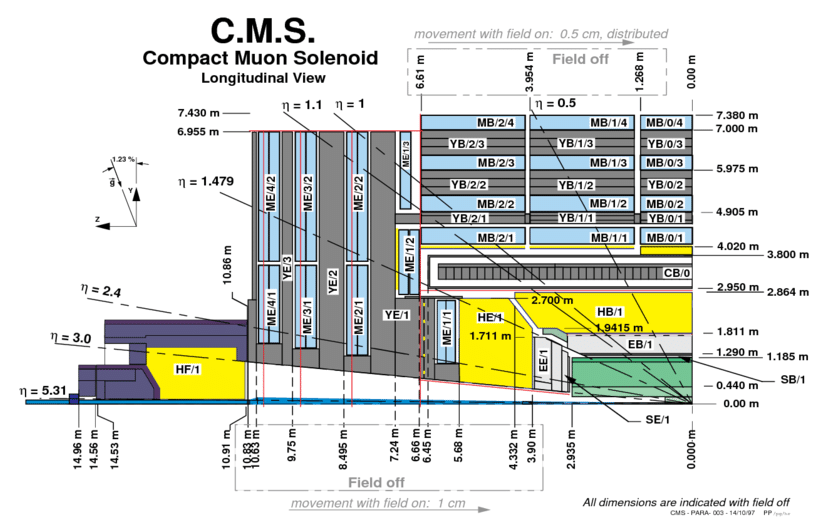
\includegraphics[width=\textwidth]{\PhDthesisdir/plots_and_images/from_CMS_alignment_photodetectors/CMS-eta-ranges.png}
\caption[Vue longitudinale d'un quadrant du détecteur CMS.]{Vue longitudinale d'un quadrant du détecteur CMS~\cite{CMS_alignment_photodetectors}. Les directions correspondant à quelques valeurs de pseudo-rapidité sont illustrées et des mesures de distances par rapport au centre du détecteur, lieu des collisions, sont indiquées. Le sol de la caverne présente une inclinaison de \SI{1.23}{\%} par rapport à la direction de la gravité locale $\vec{g}$, ce que montre le schéma à gauche.}
\label{fig-chapter-LHC-section-CMS-subsec-overview_and_coordinates-CMS-eta-ranges}
\end{figure}